\documentclass[10pt,a4paper]{article}
\usepackage{fontspec}
\defaultfontfeatures{Mapping=tex-text}
\usepackage{xunicode}
\usepackage{xltxtra}
%\setmainfont{???}
\usepackage{amsmath}
\usepackage{amsfonts}
\usepackage{amssymb}
\begin{document}


\section*{Example}


The following is a very simple example for the query of an element (see fig. \ref{fig:topodallidle}), that is then exported as a CSV-file (see fig. \ref{fig:topodallcsv}), which is in turn used to generate a map (see \ref{fig:topodallmap}). A query was made using the single lexeme \emph{Dall} `valley' in this exact graphematic rendering.


\begin{figure}[h]
%\includegraphics[scale=1.2]{images/spacegramm_01_helperich.pdf}
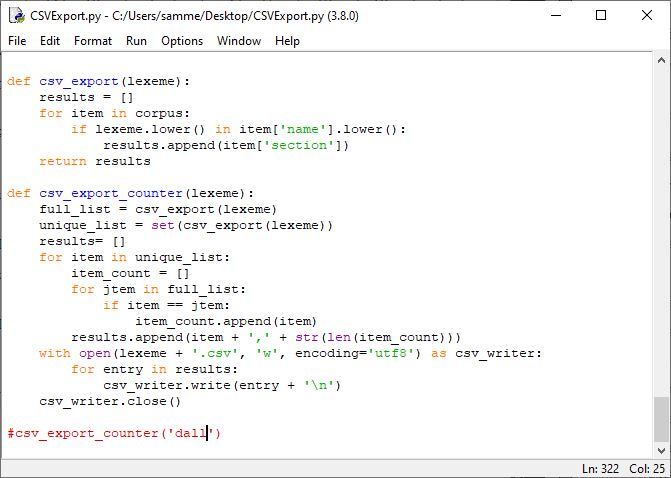
\includegraphics[width=\linewidth]{images/topo_dall_idle.jpg}
\centering
\caption{Code and query for CSV Export in Python's IDLE editor} \label{fig:topodallidle}
\end{figure}



\begin{figure}
%\includegraphics[scale=1.2]{images/spacegramm_01_helperich.pdf}
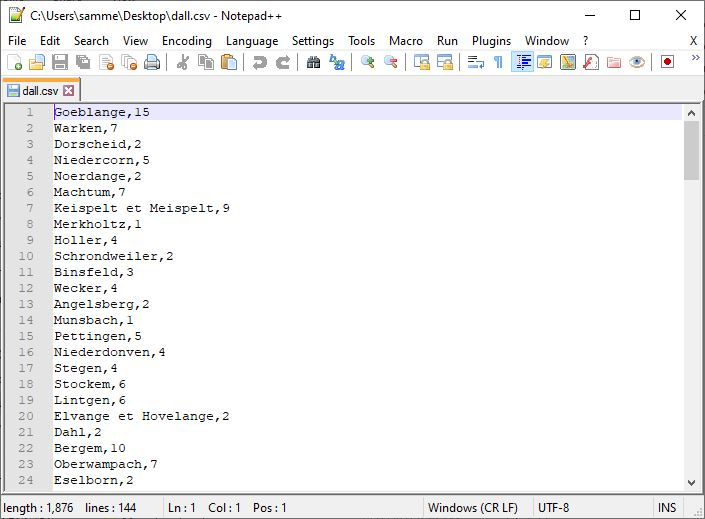
\includegraphics[width=\linewidth]{images/topo_dall_csv.jpg}
\centering
\caption{Exported CSV file} \label{fig:topodallcsv}
\end{figure}



\begin{figure}
%\includegraphics[scale=1.2]{images/spacegramm_01_helperich.pdf}
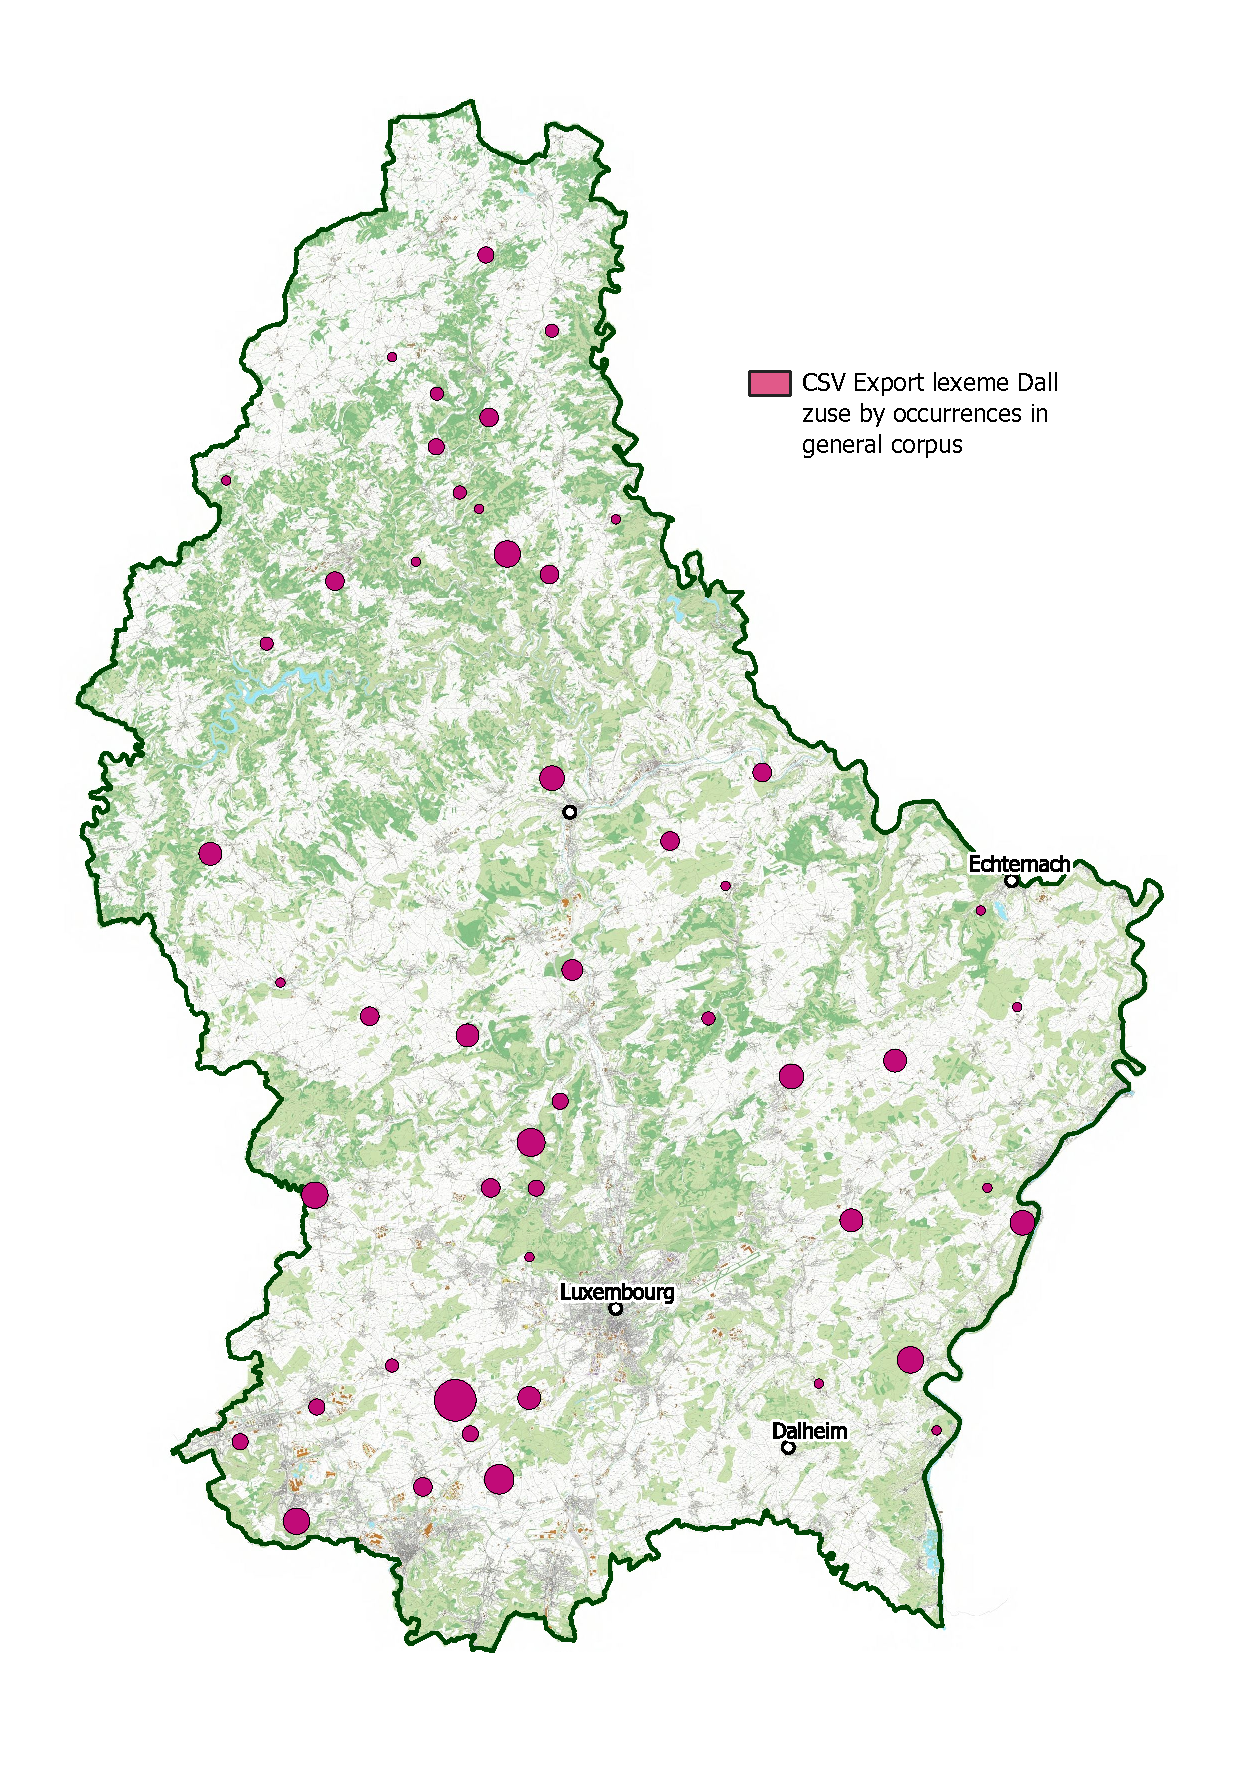
\includegraphics[width=\linewidth]{images/topolux1.pdf}
\centering
\caption{Map generated with CSV Export} \label{fig:topodallmap}
\end{figure}



\end{document}





\section*{Example}


The following is a very simple example for the query of an element (see fig. \ref{fig:topodallidle}), that is then exported as a CSV-file (see fig. \ref{fig:topodallcsv}), which is in turn used to generate a map (see \ref{fig:topodallmap}). A query was made using the single lexeme \emph{Dall} `valley' in this exact graphematic rendering.


\begin{figure}
%\includegraphics[scale=1.2]{images/spacegramm_01_helperich.pdf}
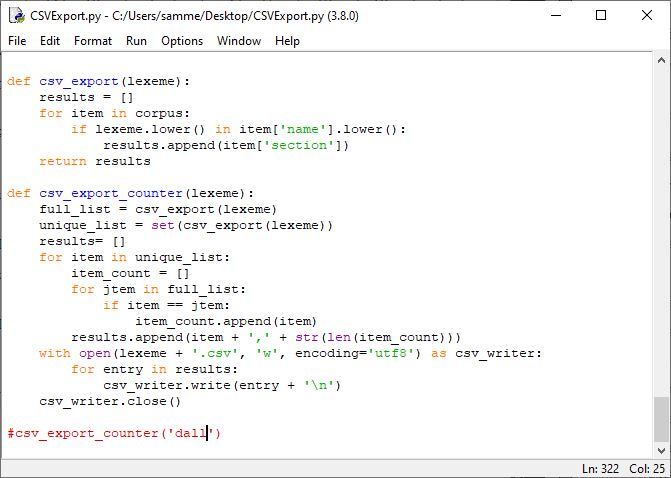
\includegraphics[width=\linewidth]{images/topo_dall_idle.jpg}
\centering
\caption{Code and query for CSV Export in Python's IDLE editor} \label{fig:topodallidle}
\end{figure}



\begin{figure}
%\includegraphics[scale=1.2]{images/spacegramm_01_helperich.pdf}
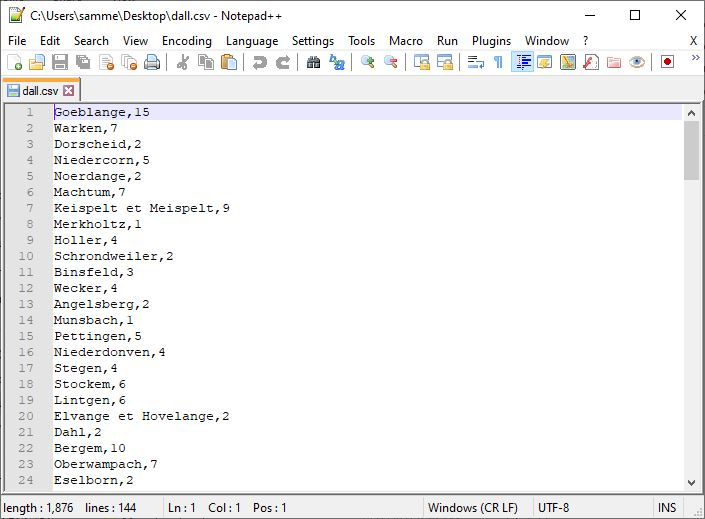
\includegraphics[width=\linewidth]{images/topo_dall_csv.jpg}
\centering
\caption{Exported CSV file} \label{fig:topodallcsv}
\end{figure}



\begin{figure}
%\includegraphics[scale=1.2]{images/spacegramm_01_helperich.pdf}
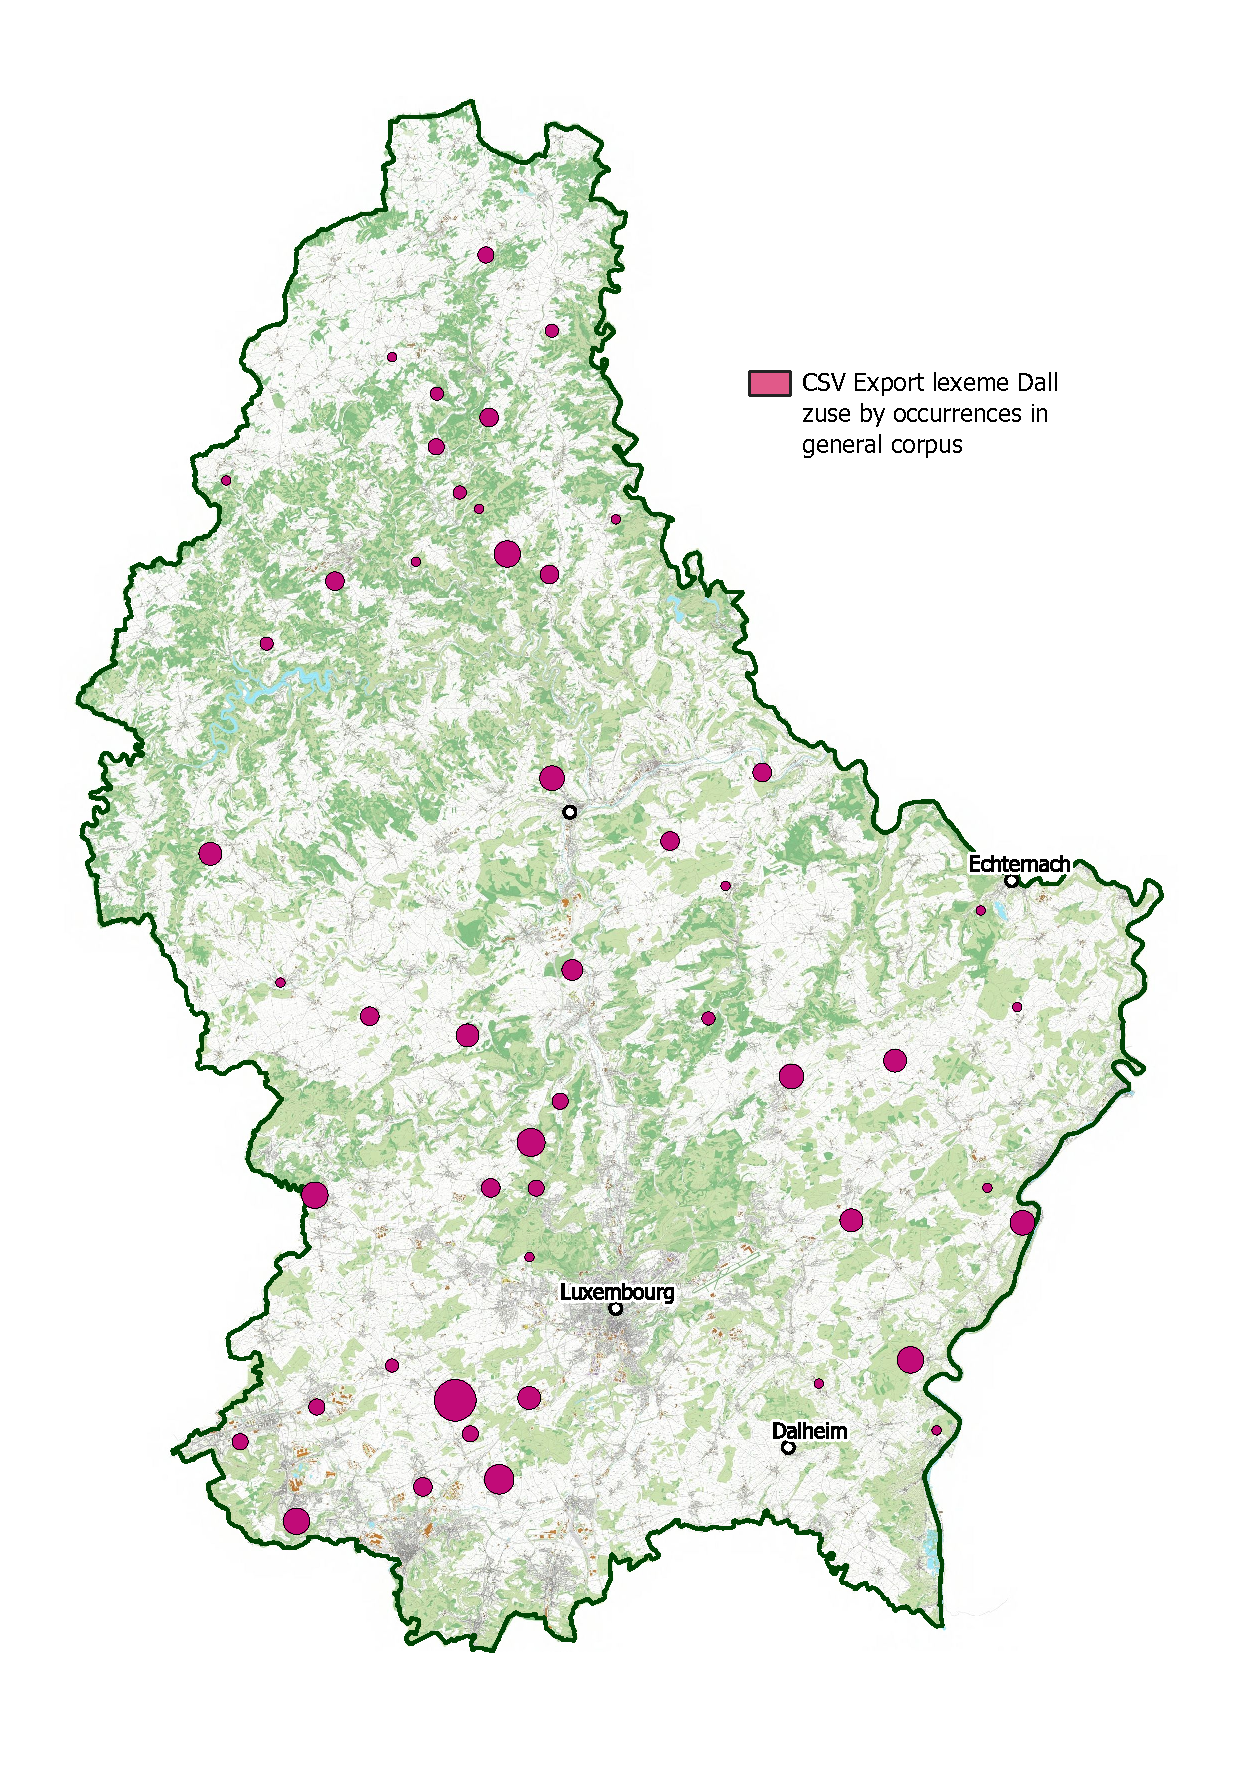
\includegraphics[width=\linewidth]{images/topolux1.pdf}
\centering
\caption{Map generated with CSV Export} \label{fig:topodallmap}
\end{figure}
